
\begin{figure}
		\begin{subfigure}{.5\textwidth}
		  \centering
		  	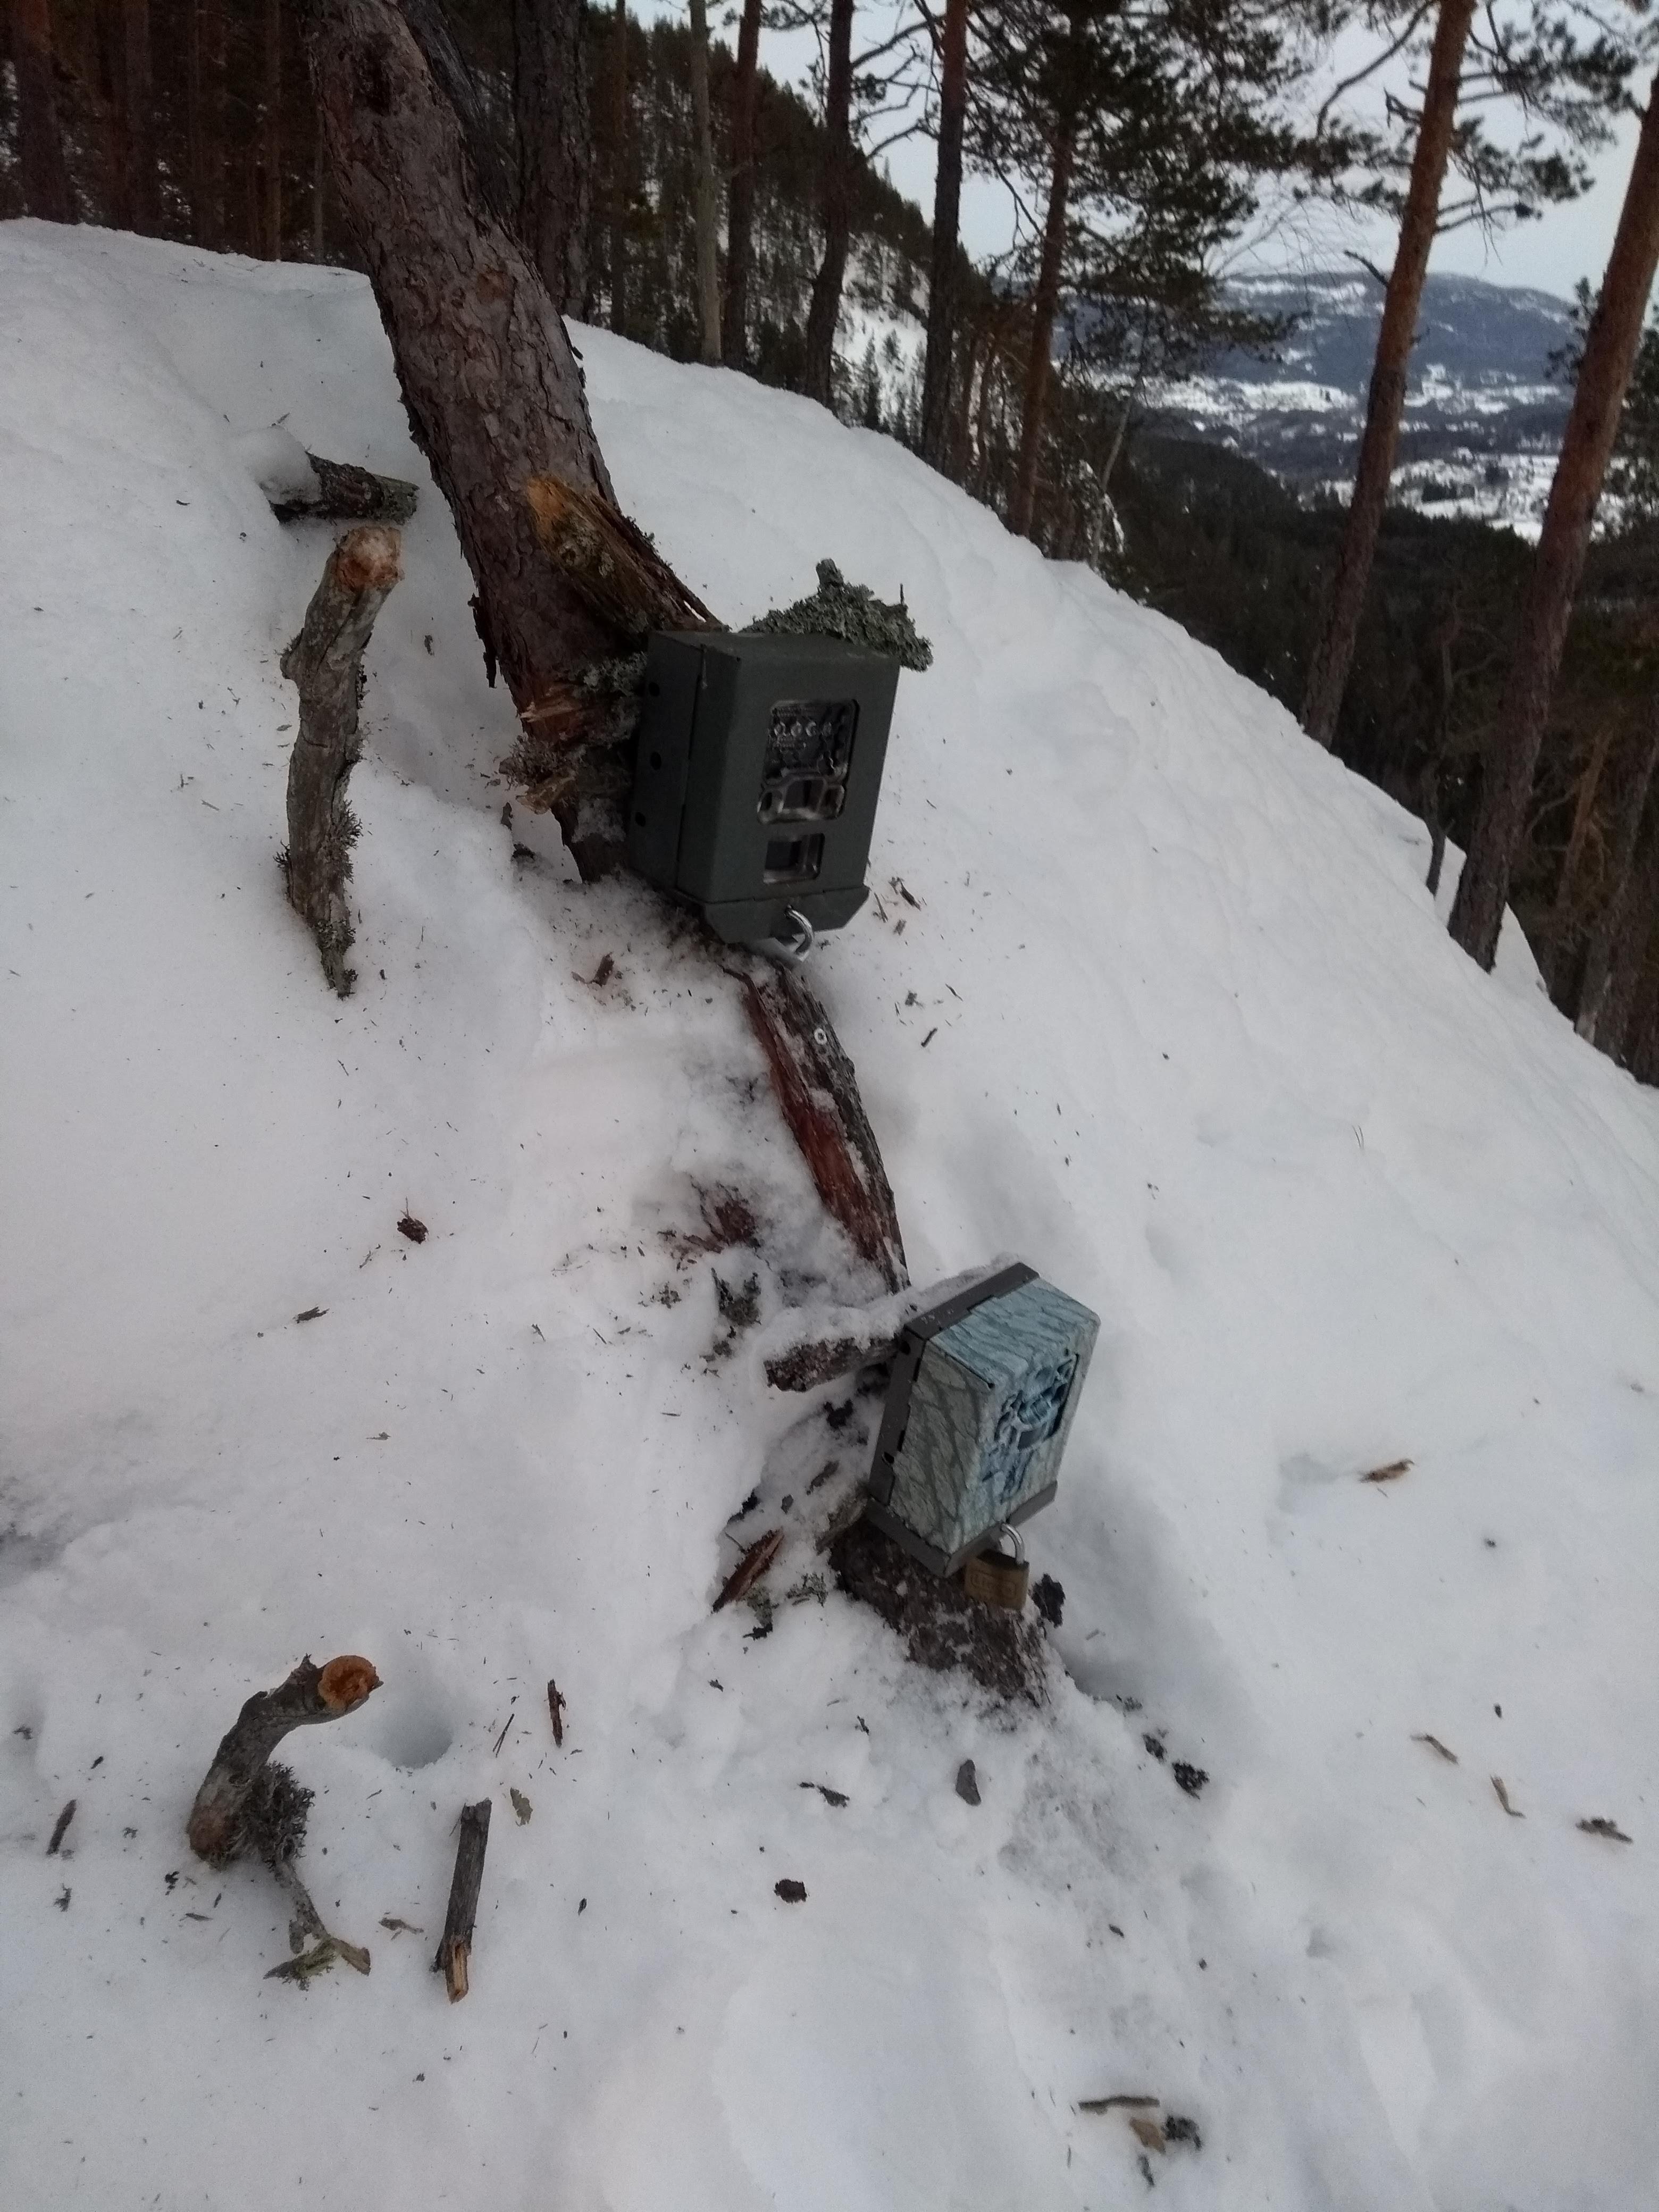
\includegraphics[width=.8\linewidth]{./img/cam_install_example/IMG_20190212_161615169.jpg}
		  \caption{Browning IR installed on fallen tree.}
		  	\label{fig:cam_ex_a}
	\end{subfigure}
		\begin{subfigure}{.5\textwidth}
		  \centering
		  	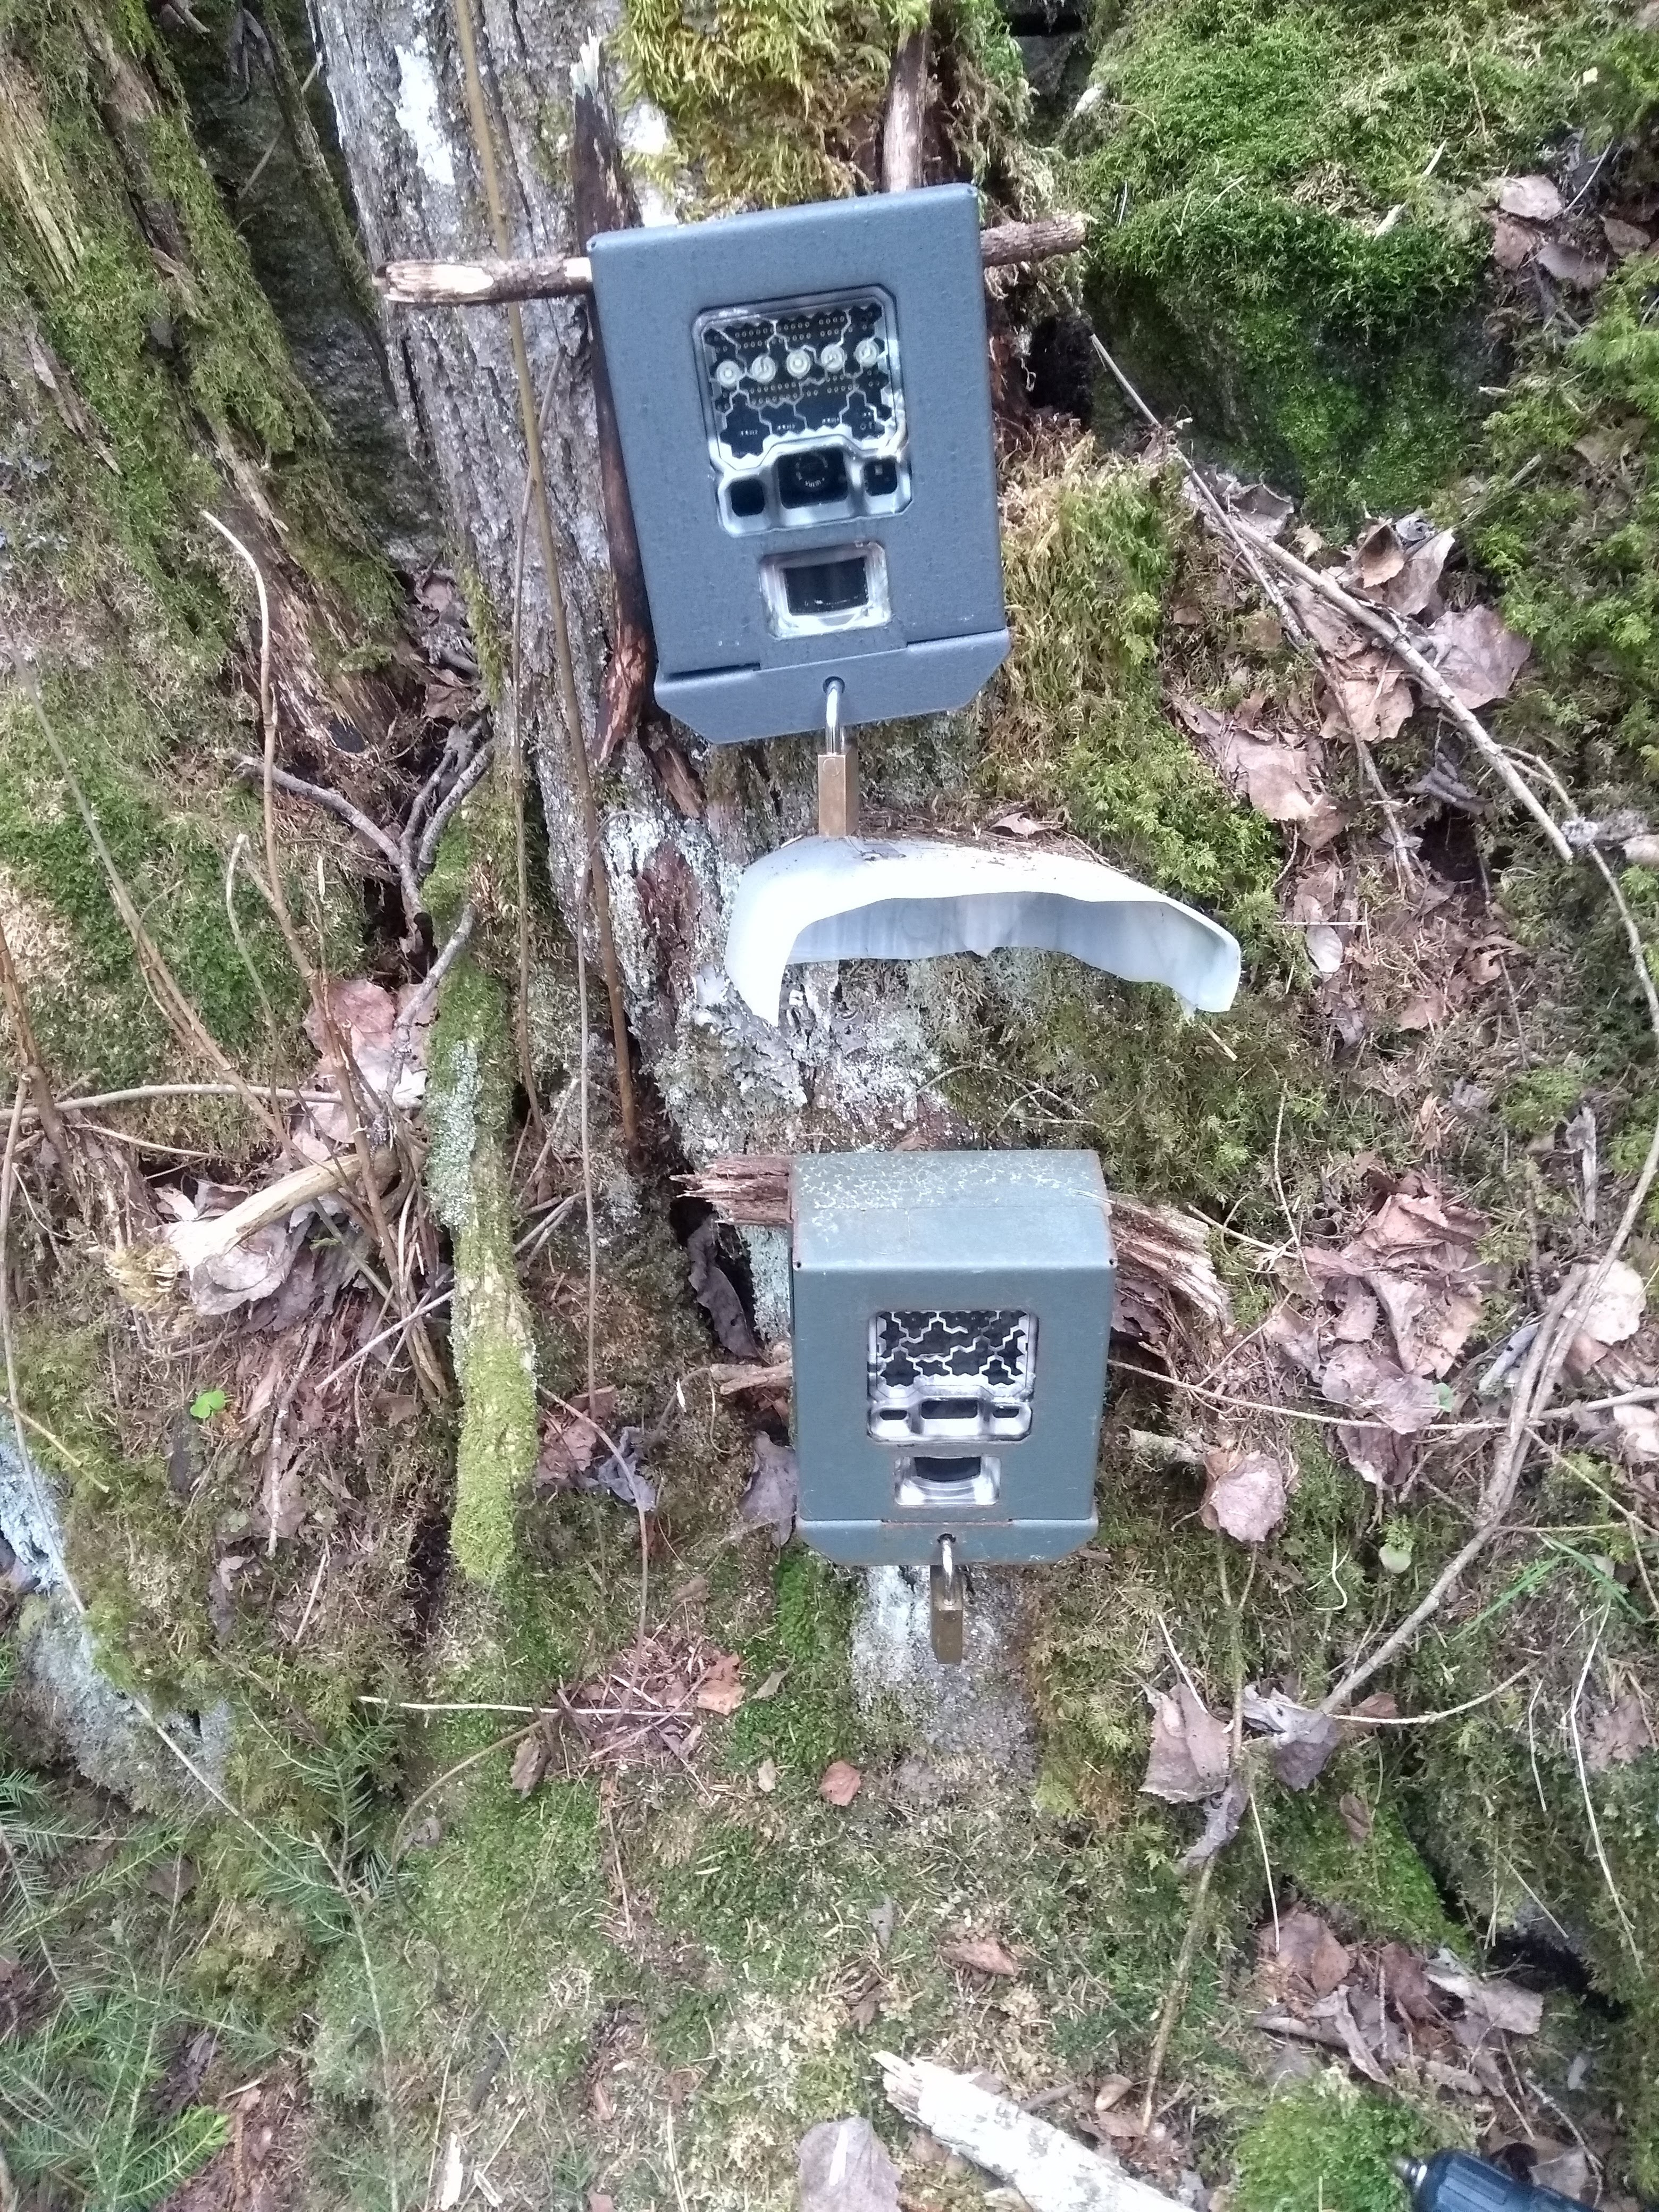
\includegraphics[width=.8\linewidth]{./img/cam_install_example/IMG_20190515_170952923.jpg}
		  \caption{Reconyx IR installed with snow cap.}
		  	\label{fig:cam_ex_b}
	\end{subfigure}
		\begin{subfigure}{.5\textwidth}
		  \centering
		  	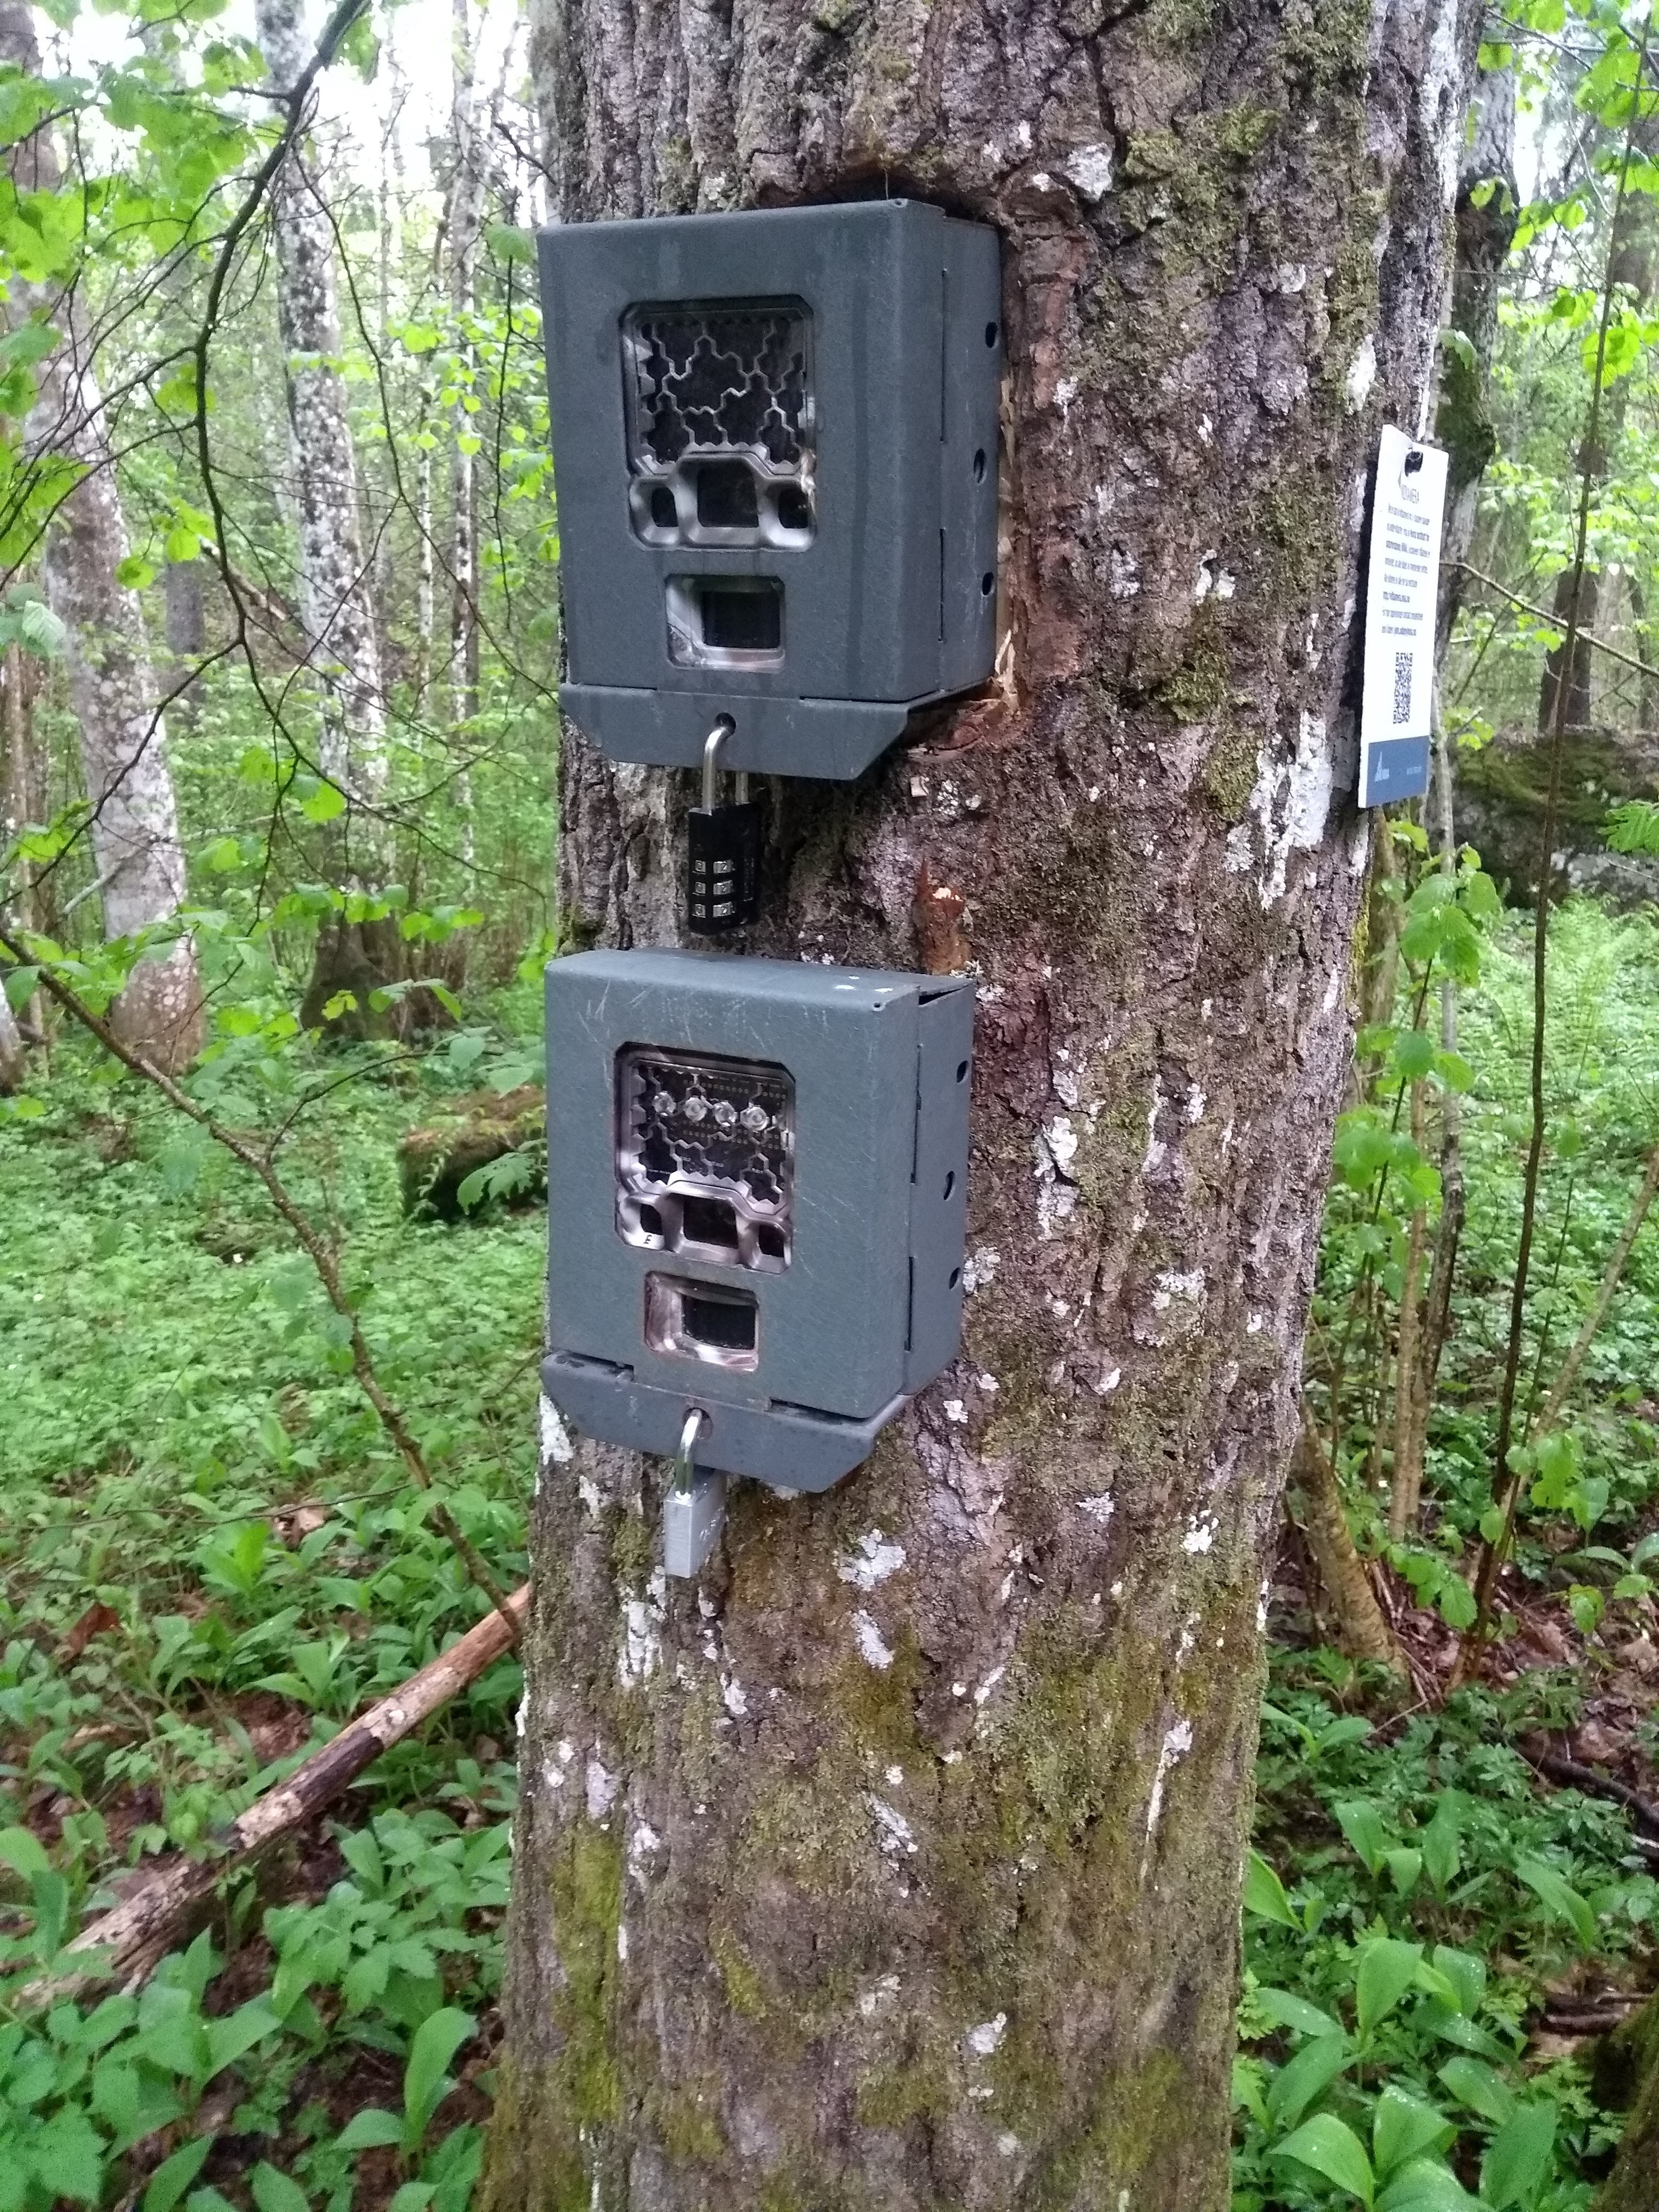
\includegraphics[width=.8\linewidth]{./img/cam_install_example/IMG_20190521_181329313.jpg}
		  \caption{Reconyx IR 160 cm above the ground.\\ Therefore, I positioned the LED underneath.}
		  	\label{fig:cam_ex_c}
	\end{subfigure}
		\begin{subfigure}{.5\textwidth}
		  \centering
		  	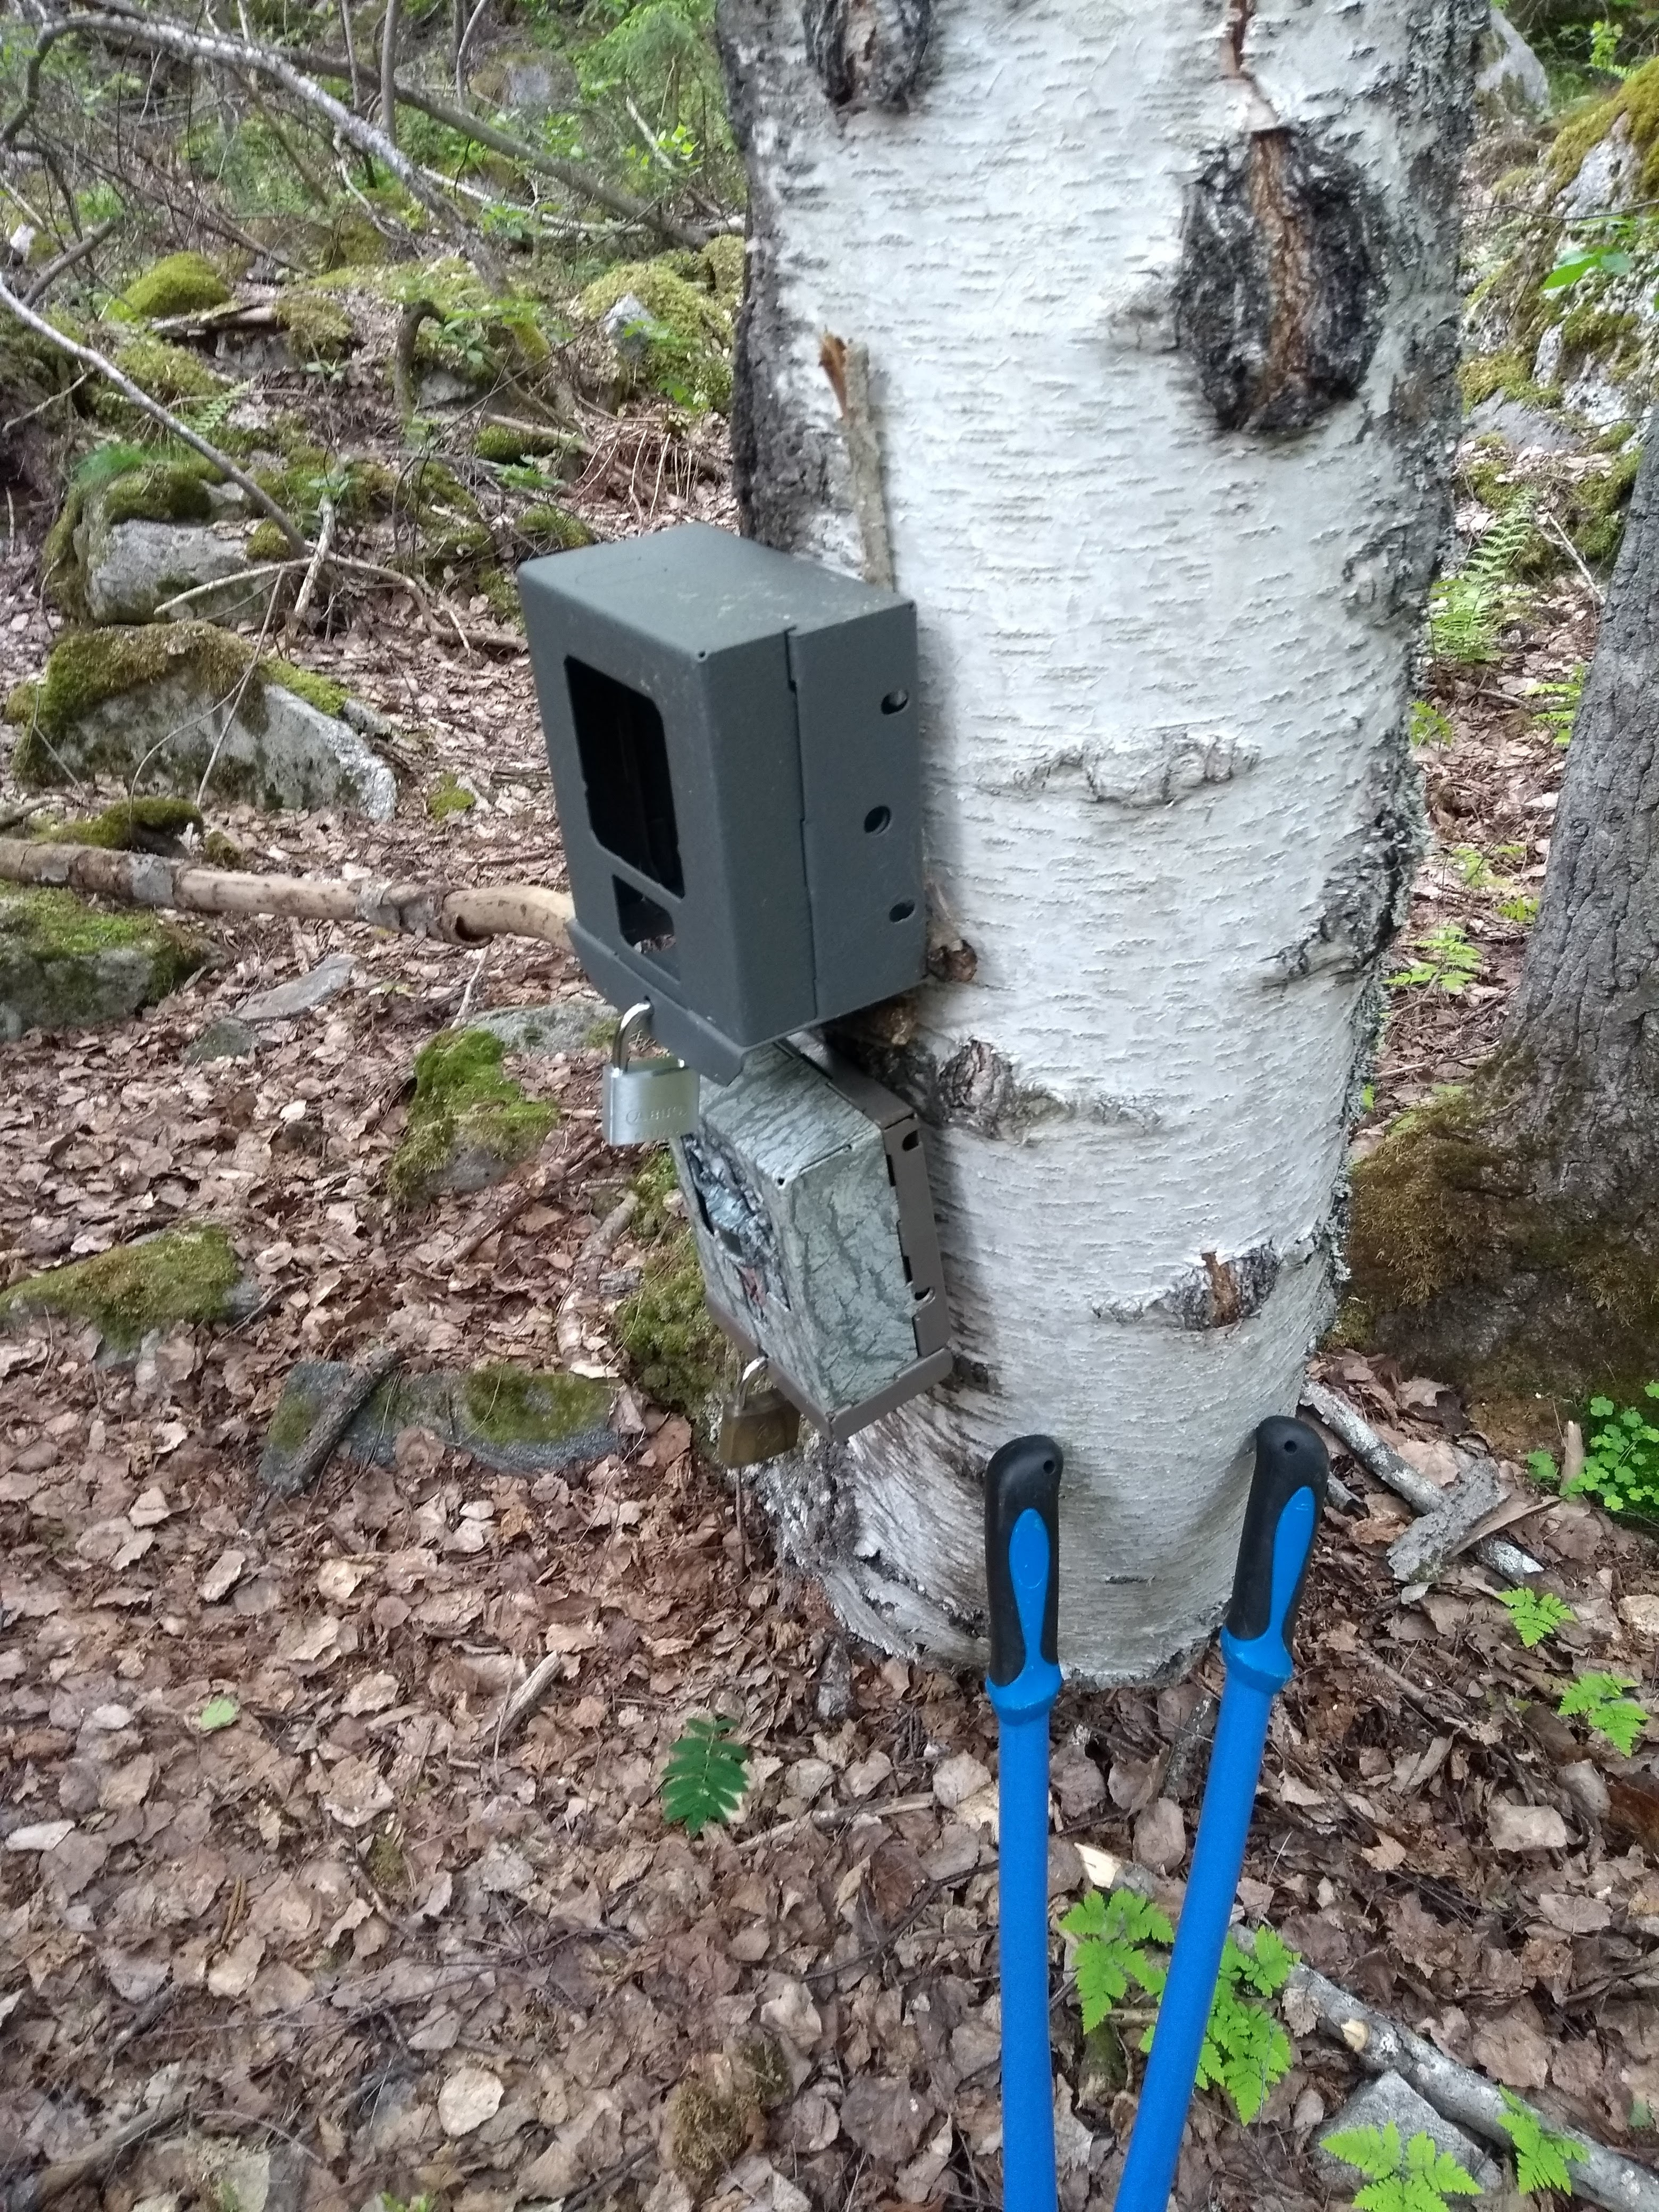
\includegraphics[width=.8\linewidth]{./img/cam_install_example/IMG_20190529_181049340.jpg}
		  \caption{Additional CT boxes remained\\ during IR periods.}
		  	\label{fig:cam_ex_d}
	\end{subfigure}
		\caption[Examples of camera setups]%
		{Examples of camera setups \par \small The preinstalled IR cameras varied in the way they were set up. Lower cameras were IR, upper cameras were white LED at all sites except the one in example c.}
	\label{fig:cam_ex_main}
\end{figure}


